\chapter{Turbulence and Instability}
\label{c_turb_and_inst}

Turbulence is a ubiquitous phenomenon in fluids that has been recognized and studied for centuries. It is often called the last unsolved problem in classical physics because we cannot predict in detail how or why
turbulence occurs or fully predict its behavior. It is, however, extremely important to gain an understanding of it in laboratory plasmas and magnetically confined
fusion devices because it causes increased particle and energy
transport. This is not necessarily a good or bad property as far fusion devices are concerned on the whole -- better energy confinement is needed in the core but not in the scrape-off-layer,
while good particle confinement is needed in the scrape-off-layer but not in the core. Nevertheless, an enhanced understanding of plasma turbulence would allow for greater control to achieve
the properties needed for fusion and would allow for greater prediction of future machine performance.

\section{Paradigms of Turbulence}
\label{s_turb_paradigms}

In the past, researchers thought that turbulence was a random process that could only be described in a statistical manner~\cite{tennekes1972}. This is the classical view of turbulence.
This view, however, contradicted the also widely-held belief that the Navier-Stokes equations can fully describe turbulent flow in neutral fluids~\cite{mcdonough04}. 
This is contradictory because the Navier-Stokes equations are deterministic (assuming yet unproven existence of the solutions), so they cannot possibly describe a random flow.
Apparently, some scientists in the first half of the 20$^{th}$ century didn't regard this as a problem, while others took this as a cue to abandon the fully equation-based approach 
to studying turbulence~\cite{tennekes1972}. In any case, statistical theory dominated. 
Not until the 1970's was a deterministic theory of turbulence formulated. Nevertheless, the deterministic approach does
not mean that turbulent statistics are useless because even though the turbulence is not random, it can still be stochastic. I note that random and stochastic are often used interchangeably,
but formally, stochastic refers to a variable whose autocorrelation decays exponentially fast to zero. Thus, a deterministic system may be stochastic, but not random. And stochasticity
is sufficient for statistical tools to be effective~\cite{mcdonough04}. Even non-stochastic systems are often described statistically, although they often have more informative descriptions as well.

In any case, certain statistical descriptions are still widely accepted in the fluid and plasma communities. Perhaps the most important is Kolmogorov's theory (K41 theory) of high Reynolds number
small scale turbulence~\cite{Kolmogorov1941,tennekes1972}. 
It's based on the idea that large scale turbulent structures (eddies) are driven by instability at the largest scales (the system and integral scales), 
which then drive eddies of smaller scales in a cascade process. The cascade process occurs in the inertial wavenumber range, which has a power law spectrum with index of $-5/3$. When energy
cascades down to the Kolmogorov scale, viscosity takes the energy away from the eddies, thermally transferring it to the fluid. I show a typical Kolmogorov spectrum in Fig.~\ref{kolmogorov}.

\begin{figure}[!ht]
\centerline{\includegraphics[]{kolmogorov}}
\caption{Kolmogorov energy spectrum}
\label{kolmogorov}
\end{figure}

The modern view of turbulence is that it is deterministic~\cite{mcdonough04}. Most of the plasma community readily accepts this as evidenced by its use of deterministic equation sets and simulations
used to model plasma turbulence. The first clue that deterministic equations could describe something as apparently random as turbulence was provided by Lorenz in 1963~\cite{lorenz1963}.
He showed that a deterministic equation derived from the Navier-Stokes equations could exhibit random-looking behavior, and that it was sensitive to small changes in initial conditions.
In 1971, Ruelle and Takens showed that the Navier-Stokes equations are capable of producing chaotic solutions that are sensitive to initial conditions and are associated with the mathematical
concept of a strange attractor~\cite{ruelle1971,mcdonough04}. They also presented a sequence of transitions (bifurcations) that a flow undergoes as the Reynolds number is increased
on its way to a chaotic state: steady $\rightarrow$ periodic $\rightarrow$ quasi-periodic $\rightarrow$ chaotic. This isn't the only possible bifurcation sequence; 
in fact, some flows like Poisueille pipe flow go straight from steady to chaotic. 
In any case, it's significant that the sequence is short and finite, meaning that turbulence may occur at finite Reynolds number, and it can be understood in terms
of a strange attractor. Interestingly, Biskamp and Kaifen showed that a system of three plasma drift waves undergoes a Ruelle-Takens bifurcation sequence~\cite{biskamp1985}.

Recently, Maggs and Morales gave support to the deterministic viewpoint of plasma turbulence (in several different machines and experiments) by connecting the exponential frequency spectra
observed in many plasma experiments to a deterministic chaotic process~\cite{maggs2011,maggs2012a,maggs2012b}. Specifically, they showed that low-order deterministic dynamical systems could
produce the Lorentzian pulses in the time signal that give rise to an exponential frequency spectrum. The Lorentzian pulses are the result of a certain orbit structure surrounding
a limit cycle attractor. This showed that experimental turbulence could be explained in terms of deterministic chaos.

Anyhow, this dissertation is not primarily concerned with bifurcations or the nature of a particular strange attractor. I simply mention this to give credence to my use of a deterministic set
of dynamical equations to model the turbulence in LAPD. Furthermore, some of my results may be of use to others who wish to pursue the kinds of studies undertaken by Biskamp~\cite{biskamp1985}
and Maggs~\cite{maggs2012a}. Also, I will occasionally refer to cascades, stochasticity, etc., and I wanted to explain my use of these terms in advance.


\section{Instability: Turbulent Drive}
\label{s_nlin_stability}

The focus of this dissertation is on the specific process that drives turbulence in LAPD and possibly many other devices. Turbulence is dissipative and therefore needs a source of energy
to sustain itself. Generally, this source comes from a gradient in a steady (equilibrium) variable such as a flow or a pressure. Fluctuations that take energy from these equilibrium
gradients often develop certain unstable mode structures that continue to take energy indefinitely. The details of these instabilities are important for understanding the onset of turbulence
and the structure of turbulence. Both the neutral-fluid community and the plasma community have studied instabilities in great depth.

\subsection{Linear Instabilities Abound in Plasmas}
\label{s_lin_inst_plasmas}

Linear instabilities are those that can grow from infinitesimally small fluctuations about an equilibrium. They can be calculated by linearizing a dynamical equation set about an equilibrium, where
at least one equilibrium profile has a finite gradient. A linear dynamical system can be written in the form

\beq
\label{dyn_sys_lin}
\pdiff{{\bf v}}{t} = {\bf M v}
\eeq
where ${\bf v}$ is a vector of independent variables that describe the state of the system and ${\bf M}$ is a matrix of coupling coefficients and differential operators. If the equations are
coupled, ${\bf M}$ is not diagonal. With ${\bf v}$ having an exponential time dependence, this equation is an eigenvalue problem, with (generally complex) eigenvalues $\gamma_i$
and eigenvectors $\bm{\xi}_i$, which are linearly independent. If any of the eigenvalues sit in the right half of the complex plane, their associated eigenvectors will grow exponentially
from noisy infinitessimal perturbations to the equilibrium. In this case, the system is linearly unstable. Now although having an equilibrium profile with a finite gradient is a necessary
condition for linear instability, it is not sufficient. At least one of the eigenvalues must have a positive real part. This is why so much effort goes to calculating linear plasma systems,
testing for linear instability.

In general, plasma physics has so many more types of equilibrium gradients and physical processes than neutral fluids, that there are many more linear plasma instabilities than
linear neutral fluid instabilities. Plasmas have linear instabilities due to density gradients, temperature gradients, velocity gradients, current gradients, magnetic field curvature,
and non-Maxwellian velocity-space features to name a few~\cite{wesson2004,chen2006}. 
Linear plasma instabilities can be collisional, collionless, electrostatic, electromagnetic, ionization-related, sheath-induced, etc. The shear number of instabilities can be overwhelming.
In physical systems, any number of linear instabilities can be present at the same time, combining with each other, with some being more significant than others. Often times, it can take
great effort to identify a particular linear instability with particular properties that is responsible for turbulence in a given situation. This can be important if one wants to create reduced
models or if one wants to be able to predict the type of turbulence that will occur in future machines. Unfortunately, however, this isn't even the entire story as turbulence is inherently nonlinear,
opening the door for even more instabilities.

\subsection{Supercritical Stability and Subcritical Instability}
\label{subcritcal_supercritical}

While the plasma community has focused much attention on linear stability of various plasma systems, the neutral-fluid 
community has long been aware that nonlinear stability effects are crucial to explaining observed transitions from laminar to turbulent flow~\cite{krommes1999}.
The foundations of the theory of nonlinear hydrodynamic stability were laid by Landau~\cite{landau1944,landau1959}. While his ideas have required much elaboration, qualification, and application,
they still contain many ingredients of modern day theory. I outline some of those ideas, following the treatment in Drazin and Reid~\cite{drazin1981}.

Landau began with the linear theory of stability of a steady flow, which has a spectrum of linearly independent eigenmodes, each with growth rate $\sigma$. For some dimensionless parameter $R$ 
(generally the Reynolds number in neutral fluids), when $R < R_c$, all modes have $\sigma < 0$. As $R$ increases above $R_c$, one mode becomes unstable with $\sigma > 0$, where 
$\sigma \sim R - R_c$ for $|R-R_c| \ll 1$.
He described the evolution of the amplitude $|A|$ of the most unstable or least stable mode by what is now called the Landau equation:

\beq
\label{landau_eqn}
\diff{|A|^2}{t} = 2 \sigma |A|^2 - l |A|^4
\eeq
where $l$ is the Landau constant and the $l |A|^4$ term is the nonlinearity. Landau's equation admits an analytic solution given an initial condition, making it easy to explore. 
Several different qualitative scenarios arise depending on the signs and magnitudes of $\sigma$ and $l$. If $l>0, \sigma>0$, as $t \rightarrow \infty, |A| \rightarrow (2 \sigma/l)^{1/2}$ no matter
the value of the intial condition $A_0$. This value of $A_e \equiv (2 \sigma/l)^{1/2}$ is called a fixed point attractor with a basin of attraction consisting of all values of $A_0$
since any initial state asymptotically evolves to it. Note that the linear problem
is unstable because $|A| \rightarrow \infty$ as $t \rightarrow \infty$, but the nonlinear problem is stable in that it evolves to a finite value as $t \rightarrow \infty$. This is called
supercritical stability. If $l>0, \sigma<0$, as $t \rightarrow \infty, |A| \rightarrow 0$ for both the linear and nonlinear problem. Here, the point $|A|=0$ is the fixed point attractor. 
The situation is rather simple for
$l>0$ and the bifurcation diagram for this is shown in Fig.~\ref{bifurcation_diagrams} a). The branching of the curve of the equilibrium solutions at $R = R_c, |A| = 0$ is called a bifurcation.

On the other hand, if $l<0, \sigma>0$, both the linear and the nonlinear problem are unstable with the nonlinear problem growing super-exponentially in time, becoming infinite at finite time.
Such a situation is unphysical, and the Landau equation is too simple in this case. The most interesting and most commonly studied case is when $l<0, \sigma<0$. If $A_0 < A_e$, the solution
decays to zero as $t \rightarrow \infty$. However, if $A_0 > A_e$, the solution is unstable and breaks down at finite time. This means that the system is unstable only when the initial
condition has a finite amplitude, which is in contrast to a linear instability, which is unstable to infinitesimal initial perturbations. Finite amplitude instabilities are called nonlinear
instabilities. Fig.~\ref{bifurcation_diagrams} b) depicts the bifurcation diagram
for the case of $l<0$. In this figure, $R_G$ represents a Reynolds number below which the unstable bifurcated solution doesn't exist. This isn't a part of the Landau equation, but Landau
suggested that this should be the case. 

Furthermore, unlike in the supercritical case, the subcritical case contains regions ($R>R_G$) where the unstable solution is not bounded by a higher
region of stability, indicating that the solutions become infinite. In reality, other nonlinear effects due to terms not included in the Landau equation don't allow mode amplitudes to become
infinitely large, and the flow can become turbulent. Now the subcritical case is so interesting because it allows for instability and turbulence when a system is linearly stable. This seems
to be the case in several different kinds of flows. Landau asserted that Poiseuille pipe flow is an example of this~\cite{landau1944}. 
Poiseuille pipe flow, which is flow with a parabollic velocity profile, is linearly stable for all $R$, so that $R_c = \infty$. 
But experimentally, it is known that for $R = R_G \sim 2000$, it becomes unstable to finite disturbances. Plane Couette flow (flow with linear velocity profile between two infinite moving planes)
is another example of this. Plane Poiseuille flow, also admits subcritical instability, but it has a finite $R_c$, so it's more representative of Fig.~\ref{bifurcation_diagrams} b)~\cite{trefethen1993}.

\begin{figure}[!ht]
\centerline{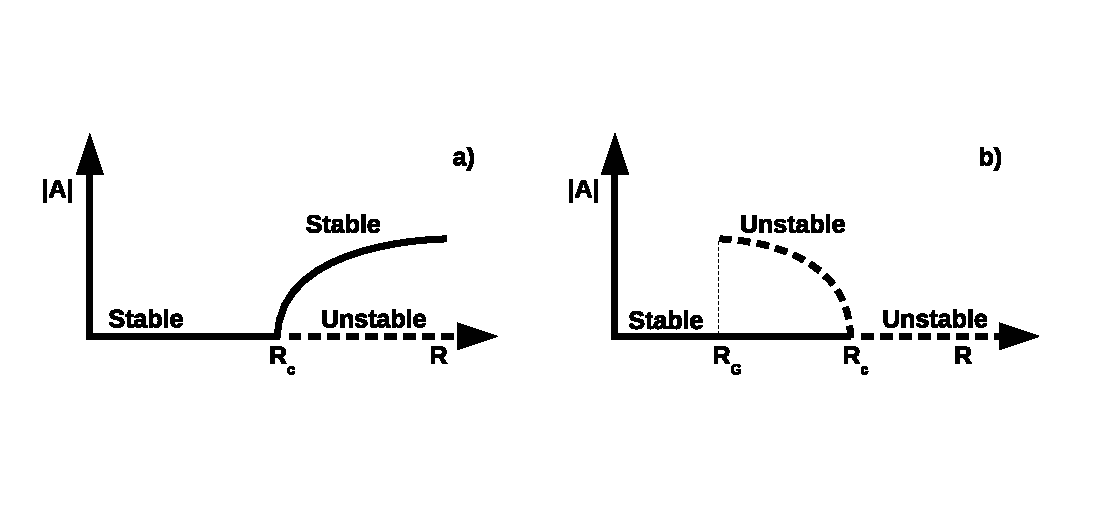
\includegraphics[width=\textwidth]{bifurcation_diagrams}}
\caption{Supercritical and subcritical bifurcation diagrams}
\label{bifurcation_diagrams}
\end{figure}


\subsection{Non-normality, Transient Growth, and Subcritical Turbulence}
\label{s_nonormality}

Subcritical instability is especially unintuitive when one considers cases in which the nonlinearities of the equation set are energetically conservative, which is typical. Then, only
the linear terms in the equations can extract energy from the equilibrium gradients. It seems reasonable that when all of the linear eigenmodes of a system are stable, there shouldn't be
any instability. This makes subcritical instability a mysterious phenomenon. However, several neutral-fluid researchers in the early 90's explained the mechanism behind linear subcritical
growth~\cite{gustavsson1991,butler1992,reddy1993,reddy1993b,trefethen1993,henningson1994,henningson1996}. The mechanism requires that the eigenvectors of the linear system be nonorthogonal.
In other words, the linear operator matrix (like ${\bf M}$ in Eq.~\ref{dyn_sys_lin}) must be non-normal. 
Such non-normality is a necessary condition for sustained subcritical turbulence in systems with conservative nonlinearities.

I illustrate the mechanism behind sustained subcritical turbulence with a simple diagram in Fig.~\ref{vector_diagram} representing a two-dimensional two-state system. 
I start in Fig.~\ref{vector_diagram} a) with two 2D linear eigenvectors that are not orthogonal to one another, but are largely anti-parallel with a $30^o$ angle between them. 
I give them each a starting amplitude so that they form a leg and a hypotenuese of a 30-60-90 triangle. The sum of these vectors, which is the other leg, is the initial state of the system.
The squared length of this is the energy of the system. Note that the total energy of the system is $|{\bf u} + {\bf v}|^2 = |{\bf u}|^2 + |{\bf v}|^2 + 2 {\bf u} \cdot {\bf v}$. So since the
eigenvectors are nonorthogonal, the total energy of the system is not just the sum of the individual energies of the eigenmodes ($|{\bf u}|^2 + |{\bf v}|^2$), but it includes an interaction
term ($2 {\bf u} \cdot {\bf v}$) that can be positive or negative.

Now, in Fig.~\ref{vector_diagram} b), I show the result of evolution of the linear system. Linearly, since the vectors are eigenvectors, 
they grow or decay exponentially at given rates $\gamma_u, \gamma_v$. And since I am
interested in the subcritical case, I give both of the vectors negative growth rates. Furthermore, ${\bf u}$ has much smaller damping rate than ${\bf v}$. After a certain amount of time, under
purely linear action -- where each vector decays at its characteristic decay rate -- the system resides in the state shown in Fig.~\ref{vector_diagram} b). Note that I have changed the scales on
the axes because the triangle has become much smaller. Perhaps surprisingly, even though both vectors ${\bf u}$ and ${\bf v}$ have decayed and have smaller magnitudes than they did in 
Fig.~\ref{vector_diagram} a), the total energy of the system (the green line) has grown! Clearly, the reason is that the interaction energy between the two vectors has become less negative.
Moreover, if the system were to continue evolving linearly, the total energy would eventually decay as the vectors become smaller. Therefore, the growth of the total energy from a) to b)
is called transient growth. One may wonder where this transient energy comes from. The answer is that the energy comes from the equilibrium gradients -- the same as unstable linear eigenvectors.
So systems in which the fluctuations are made up of only nonorthogonal stable linear eigenvectors can transiently grow in energy before decaying. At small times, the growth has been shown to be
algebraic, meaning it is proportional to time~\cite{waleffe1995}. This is in contrast to growth by unstable linear eigenmodes, which is exponential in time.

Now the linear growth in non-normal linearly stable systems is only transient, but the nonlinearities in the full nonlinear systems can take this transiently injected energy, mix it around,
and sustain the fluctuation energy or sustain the turbulence indefinitely. In Fig.~\ref{vector_diagram} c), I show how the nonlinearities, which conserve the total energy, can mix the energy
between individual modes and the interaction energy. The nonlinearities can essentially prop up the linear eigenvectors individual energies without injecting net energy into the system.
Finally, Fig.~\ref{vector_diagram} d) shows linear decay of the eigenvectors, bringing the system back to its original state with its original energy. Altogether, this is the basic
mechanism of subcritical instability or self-sustained subcritical turbulence in systems with conservative nonlinearities. It is basically a linear mechanism, but it requires nonlinearity to
sustain or bootstrap itself.
Although my simple diagram makes it seem as though the transient growth mechanism is rather weak
(amplifying the total energy from 25 to 36), the mechanism can amplify energies by factors of several thousand in realistic systems~\cite{gustavsson1991,butler1992}.

\begin{figure}[!ht]
\centerline{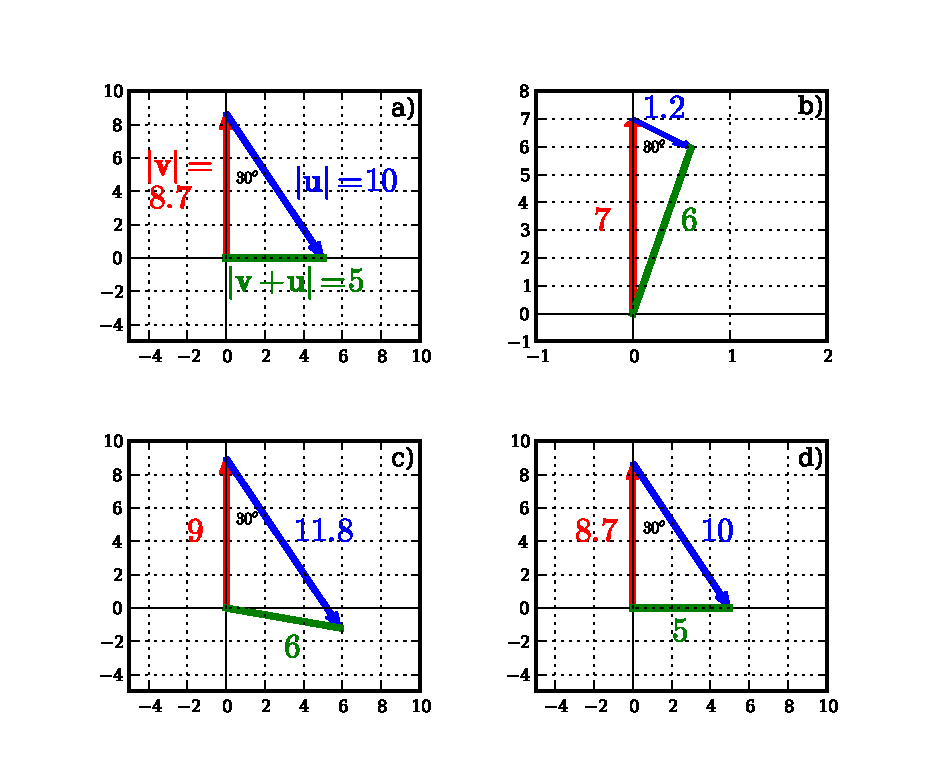
\includegraphics[]{vector_diagram}}
\caption{Non-normal subcritical instability diagram}
\label{vector_diagram}
\end{figure}
